\documentclass[article,12pt,oneside,a4paper,english,brazil,sumario=tradicional]{abntex2}
\usepackage[brazil]{babel}
\usepackage[utf8]{inputenc}
\usepackage[T1]{fontenc}
\usepackage{amsmath}
\usepackage[pdftex]{graphicx}
\usepackage{helvet}
\usepackage{url}
%\usepackage{fancyheadings}
%\usepackage{lastpage}
\usepackage{indentfirst}
\usepackage{color}
\usepackage{float}
\usepackage{lscape}
\usepackage{cancel}
\usepackage[brazilian,hyperpageref]{backref}
\usepackage[alf]{abntex2cite}

%\usepackage{layout}
\usepackage[margin=15pt,font=small,labelfont=bf,labelsep=endash,centerlast]{caption}

\renewcommand{\familydefault}{\sfdefault}
%\renewcommand{\headrulewidth}{0pt}
\newcommand{\relatnum}{XYZ ABC-DEF}


\setlength{\oddsidemargin}{-10pt}
\setlength{\topmargin}{18pt}
\setlength{\headheight}{12pt}
\setlength{\headsep}{34pt}
\setlength{\marginparsep}{0pt}
\setlength{\textheight}{214mm}
\setlength{\textwidth}{17cm}
\setlength{\footskip}{0pt}
\setlength{\marginparwidth}{0pt}

\linespread{1.3}
\setcounter{topnumber}{5}
\setcounter{bottomnumber}{5}
\setcounter{totalnumber}{10}
\renewcommand{\topfraction}{1}
\renewcommand{\bottomfraction}{1}
\renewcommand{\textfraction}{0}
\renewcommand{\floatpagefraction}{0.8}
\setlength{\floatsep}{15pt}
\setlength{\textfloatsep}{20pt}
\setlength{\parskip}{6pt}
\setlength{\parindent}{1.25cm}



\newcommand{\p}[1]{\ensuremath{ \mathbf{#1}}}    % \pr vem de preto
\newcommand{\lra}{\ensuremath{\longrightarrow}}
\newcommand{\qrq}{\ensuremath{\quad\lra\quad}}
\newcommand{\qqrq}{\ensuremath{\qquad\lra\qquad}}
\newcommand{\wt}[1]{\ensuremath{\widetilde{#1}}}
\newcommand{\mcal}[1]{\ensuremath{\mathcal{#1}}}
\newcommand{\pd}{\ensuremath{\partial}}
\newcommand{\ol}[1]{\ensuremath{\overline{#1}}}
\newcommand{\bigO}[1]{\ensuremath{\mathcal{O}\left(#1\right)}}
\newcommand{\us}{\ensuremath{u_*}}

\titulo{Escalas, Modelos e Semelhança}
\autor{Paulo José Saiz Jabardo}
\date{2022}



\begin{document}
%\layout
%\renewcommand{\thepage}{\roman{page}}
%\lhead{}
%\chead{}
%\rhead{{\footnotesize Relatório Técnico n$^o$~\relatnum~-~\thepage}}
%\rhead{{\footnotesize \thepage}}
%\lfoot{}
%\cfoot{}
%\rfoot{}
%\pagestyle{fancy}

\imprimirfolhaderosto


\section{Um problema simples mas nem tanto}
\label{sec:intro}

Vamos começar com um problema simples: o que cai mais rápido, uma bola de boliche ou uma pena?

A resposta a esta pergunta vai depender de quem está respondendo. Pergunte a uma criança ou a um adulto sem boa formação científica, a resposta será a bola de boliche. Agora, se a pergunta for feita a um vestibulando ou aluno de graduação das ditas ``ciências exatas'', a resposta será contundente: ambos caem com a mesma velocidade acelerando uniformemente.

Naturalmente, o aluno de ``exatas'' está correto, não é? Qualquer um pode fazer um experimento simples para testar estas hipóteses. Infelizmente o resultado mostrará que a criança tem razão. O aluno de ``exatas'' vai reclamar que isso é injusto pois se não tivermos atrito, ele teria razão. Infelizmente a natureza não liga para estes detalhes. O homem precisou pisar na lua para observar esta solução ``correta'': \url{https://www.youtube.com/watch?v=KDp1tiUsZw8}. Não precisamos necessariamente ir para a lua: uma câmara de vácuo gigante serve como mostrou Brian Cox em \url{https://www.youtube.com/watch?v=E43-CfukEgs}.

Convenhamos, ir para a lua ou ter acesso a uma câmara de vácuo gigante não é para qualquer um. A dúvida que surge a um observador externo ao sistema educacional científico é: o que é que vocês estão fazendo???

Não, não estamos torturando nossos jovens nem fazendo pegadinhas, estamos introduzindo o método científico. Ao contrário do que se imaginaria ao ler as redes sociais e grande mídia, a ciência não é um conjunto de fatos que devem ser decorados mas sim uma abordagem sistemática para explorar o mundo. Ao se desprezar o atrito, o problema fica muito mais simples e as leis fundamentais do universo podem começar a ser exploradas. A importância de Galileu Galilei na ciência não foram os fatos que ele desvendou mas sim a sua abordagem. Um exercício intelectual onde qualquer tipo de atrito é desprezado permitiu a formular os primeiros princípios da mecânica e o resto, como sabemos,  é história.


Será que não seria melhor sermos mais preciso em nossa análise? O vídeo do Brian Cox também ajuda elucidar esta questão. Antes de soltar a bola de boliche e a pena no vácuo, ele solta na presença do ar. Por um lado, a dinâmica da pena é extremamente complexa. Mas não existe diferença perceptível na dinâmica da bola de boliche. Fazendo uma análise frame a frame da imagem chega-se a uma aceleração de aproximandamente 9.8 $m/s^2$. Para se notar qualquer diferença entre a bola de boliche caindo no vácuo e no ar seriam necessárias medições cuidadosas, algo muito mais complexo e caro.

Se no caso da bola de boliche, as diferenças são pequenas, a trajetória da pena é extremamente complexa. Observando de perto o momento em que ela é solta, observa-se que há grandes deformações das penas logo no começo (1 min e 39 s no vídeo do Brian Cox acima). Talvez se as penas fossem rígidas a coisa seria mais simples. Solta um pedaço pequeno de papel ou cartolina onde as deformações são pequenas e a trajetória continua sendo complexa. Talvez seja uma questão de simetria, o que certamente é um ponto interessante. Soltando uma placa fina, incialmente ela terá um comportamento próximo do que se observa com a bola de boliche mas não é necessário esperar muito tempo até que a complexidade apareça. Para eliminar estas dificuldades poderíamos soltar uma esfera bem leve e lisa, talvez uma bexiga, ou bola de criança ou até mesmo ma bola de ping-pong. Mesmo assim, a trajetória pode ser complexa se esperarmos um pouquinho.


Tentar analisar a trajetória exata da pena é provavelmente impossível: o problema é certamente caótico e ao se repetir o experimento, o jeitão da trajetória será o mesmo mas cada repetição terá uma trajetória única. Até mesmo caracterizar a geometria e propriedades mecânicas da pena é uma tarefa ingrata. Simplificar o problema, o que aqui chamamos de modelagem é a única saída.

Agora é possível entender a genialidade de Galileu. Atacar o problema diretamente mexe com todas as suas nuances  é um problema quase impossível mesmo nos dias de hoje onde todos (ou quase) os fenômenos envolvidos são conhecidos. O problema da queda da pena envolve tudo o que há de mais difícil  em dinâmica, mecânica dos fluidos, elasticidade, biologoia, etc. Este problema ``simples'', é muito mais complexo do que parece. Se para Galileu e Newton (e mais tarde Einstein, Heisenberg, Schrödinguer, etc) o problema era determinar os fundamentos da física, hoje em dia, mesmo conhecendo detalhadamente todos (será?) os fenômenos que ocorrem na queda da pena ainda estamos longe de prever de maneira precisa a sua trajetória. As coisas podem ser difíceis por motivos diferentes. Para Galileu, Newton, Einstein, etc a dificuldade era a física ainda não conhecida. Para nós é a enorme complexidade e a grande quantidade de detalhes presentes em qualquer problema real.

\subsection{Modelos}

Mas nem tudo está perdido. A queda da bola de boliche no ar sugere que podemos simplificar um pouco o problema e aplicar a segunda lei de Newton:
\[
m a = m g - F_a
\]
Nesta equação, $m$ é a massa da bola, $a$ é a sua aceleração, $g$ a aceleração da gravidade e $F_a$ é a força de atrito. Se $F_a = m g$, a aceleração é zero e portanto a velocidade é constante. Esta velocidade é conhecida como velocidade terminal. No entanto, se $F_a$ for pequeno, $F_a \ll mg$, o problema é muito semelhante ao problema no vácuo. 

É lógico que o problema não está resolvido: quanto vale $F_a$? Isso poderia ser obtido realizando experimentos ou calculando a partir das equações da mecânica. Um modelo comum, que será explorado a fundo adiante é:
\[
F_a = C_D A \frac{1}{2}\rho U^2
\]
onde $C_D$ é um coeficiente, $A$ é a área da seção transversal da esfera ($\pi D^2 /4$), $\rho$ é a massa específica do ar (ou qualquer outro fluido) e $U$ é a velocidade de queda. Neste modelo, com o passar do tempo, a velocidade aumenta mas com isso também aumenta a força de arrasto, reduzindo a aceleração. Se esperarmos tempo o suficiente, a força de arrasto irá se igualar com o peso e não haverá mais aceleração. Esta velocidade é conhecida como velocidade terminal. Conhecendo $C_D$, podemos estimar a velocidade terminal:
\[
U = \sqrt{\frac{2 m g}{C_D A \rho}}
\]

O segredo é não olhar com atenção demais estas equações. $C_D$ varia com a velocidade (mais precisamente com um número adimensional chamado de número de Reynolds) mas também varia com a orientação do corpo. As forças podem não estar alinhadas na vertical e variar no tempo (estas duas situações ocorrem na realidade), nenhuma bola é uma esfera perfeita  e por aí vai. Mas com cuidado e discernimento, pode-se chegar longe com estes modelos simples. Mas a realidade é muito mais complexa. Quem não se lembra das reclamações sobre a bola Jabulani na copa de 2010. Quem diria que uma bola de futebol poderia causar tantos problemas no século XXI. Nem vou mencionar o quão difícil é jogar bola com uma bexiga. Estes dois exemplos não se resumem à queda vertical de uma esfera mas mostram que a dinâmica de uma esfera em um meio fluido é mais complexo do que parece. O vídeo \url{https://www.youtube.com/watch?v=16Ci_2bN_zc} do excelente canal Veritassium entra em maiores detalhes sobre a velocidade terminal de corpos caindo.

Este modelo ainda tem um problema sério: uma bexiga com hélio ou uma bola de ping-pong dentro d'água vai ter um comportamente bem diferente. Então podemos introduzir um novo termo na equação: o princípio de Arquimedes. No entanto, agora uma nova dificuldade aparece: qual a direção da força de arrasto? Considerando a direção z como vertical para cima,

\[
m \frac{d^2 z}{dt^2} = -mg - C_D A \frac{1}{2} \rho |U|\cdot U + g m_f
\]
onde $z$ é a altura da esfera, e $m_f$ é a massa de fluido se a esfera fosse feita do mesmo fluido que o meio e pode ser escrita como $\rho\cdot g \cdot V$ onde $V$ é o volume ocupado pelo corpo. Agora temos um modelo que funciona, mais ou menos bem. Leva em consideração a força de arrasto, a flutuação e o campo gravitacional. Existe uma caixa preta que é o coeficiente de arrasto $C_D$. Todas as limitações discutidas acima permanecem mas este modelo pode fornecer várias informações interessantes. Para se resolver esta equação diferencial, precisamos das condições iniciais: No instante, $t=0$, $U=U_0$ (no nosso exemplo $U_0 = 0$) e $z=0$.

\subsection{Escalas}


Fazem parte deste modelo diferentes parâmetros, $m$, $g$, $C_D$, $A$, $\rho$ e  $V$. Estes parâmetro não são independentes. Dado um corpo rígido, existe uma relação entre volume e área. A razão entre os dois é um comprimento que no caso de uma esfera, vale
\[
\frac{V}{A} = \frac{2}{3}\cdot D
\]

Se quisermos saber a velocidade terminal, basta postular que a aceleração é zero:
\[
mg + C_D A \frac{1}{2} \rho |U|\cdot U  = g \rho V
\]
Dividindo esta equação por $g \rho V$ chegamos à seguinte relação:
\[
\left| \frac{m}{\rho V} - 1 \right| = \frac{C_D A U^2}{2 V g}
\]

Lembrando que existe uma relação entre volume e área, e definindo $L = \sqrt[3]{V}$
\[
\left| \frac{m}{\rho L^3} - 1 \right| = k \cdot \frac{U^2}{L g}
\]
onde $k$ é uma constante que depende da geometria e incorpora não apenas a razão entre volume e área mas também o coeficiente de arrasto e constante 2. Este problema, da maneira que está escrito, depende dos seguintes parâmetros:

\begin{itemize}
\item $m$ - massa do corpo
\item $\rho L^3$ - massa do fluido deslocado pelo corpo
\item $Lg$ - Dimensão vezes aceleração da gravidade
\item $k$ - um coeficiente que depende da geometria e aerodinâmica
\end{itemize}

\subsection{Parâmetros adimensionais}
Nesta última equação, os termos $\frac{m}{\rho L^3}$, $k$ e $\frac{U^2}{L g}$ não possuem unidades, ou seja, mudando o sistema de unidades o valor destas grandezas fica constante. Estas são grandezas adimensionais. Repare que neste modelo, estes parâmetros adimensionais são resultado da razão de forças - dividimos a equação original pela força de flutuação.

\subsection{Semelhança}
Estes parâmetros adimensionais, produto de manipulação simples do modelo original, tem consequências interessantes. Neste modelo, fixado os parâmetros adimensionais $\frac{m}{\rho L^3}$ e $k$, o outro parâmetro adimensional $\frac{U^2}{Lg}$ é conhecido. Podemos mudar a massa, densidade do fluido, aceleração da gravidade e dimensões do corpo mas enquanto estes parâmetros forem os mesmos, teremos um mesmo valor de $\frac{U^2}{Lg}$. Este é o resultado mais conhecido da Análise Dimensional e é essencial na condução de experimentos em escala reduzida.

\subsection{Um modelo é uma idealização do problema}
Chegamos a um modelo para a velocidade  problema da queda de um corpo. Para se chegar a este modelo utilizamos uma relação básica da dinâmica, a segunda lei de Newton e um modelo empírico para a força de arrasto de um corpo. A maneira como empregamos a segunda lei de Newton já pressupõe várias simplificações no problema como o fato da força de arrasto estar alinhado com a vertical o que sabemos não ser verdade para a queda de uma pena. Escondemos todas as dificuldades no coeficiente semi-empírico $C_D$. Sabemos que a realidade é muito mais complicada. Mas este modelo pode fornecer informações importantes. Mesmo no caso da queda de uma pena, um coeficiente de arrasto médio pode fornecer informações importantes.

Na pior das hipóteses, um modelo simples permite compreender melhor o problema real e estimar as grandezas importantes do problema, facilitando o projeto de experimentos mais sofisticados.

\subsection{Estrutura deste artigo}

Com o exemplo do corpo caindo em um meio fluido em um campo gravitacional constante, introduzimos vários conceitos como modelos, parâmetros adimensionais e semelhança. Vamos, agora, entrar mais a fundo em cada questão. Geometria simples será usada para entender melhor os parâmetros adimensionais e semelhança. Em seguida usaremos estes conceitos em alguns problemas simples com equações diferenciais conhecidas, em particular a aerodinâmica de uma esfera. Finalmente apresentaremos a análise dimensional e o teorema dos $\Pi$s de Buckingham.



\section{Um pouco de geometria}

Todo mundo sabe que a área de um quadrado é dado pelo quadrado de sua aresta, $A=a^2$. O perímetro por sua vez é um múltiplo da aresta, $P = 4\cdot a$. No caso de uma circunferência de raio $r$, $A = \pi r^2$ e $P = 2\pi r$. Em geral qualquer figura geométrica apresenta relações do tipo 
\[
\frac{A}{L^2} = k_1 \qqrq \frac{P}{L} = k_2
\]
de modo que a razão entre a área e uma dimensão característica ao quadrado é uma constante e a razão entre perímetro e esta mesma dimensão característica também é constante. 

Este tipo de relação continua valendo para figuras compostas mais complexas como a dada na figura \ref{fig:L2d} que mostra uma geometria um pouco mais complexa, composta por dois retângulos. Neste caso, a área é $A = a\cdot b + c\cdot d$ e o perímetro é $a + 2b + 2d + c$. Novamente esta figura geométrica pode ser especificada usando o lado $a$ e três parâmetros $\alpha_1$, $\alpha_2$ e $\alpha_3$ onde
\[
b = \alpha_1\cdot a, \qquad d = \alpha_2\cdot a, \qquad c = \alpha_3\cdot a
\]
A área e o perímetro desta figura geométrica são dadas por:
\[
\frac{A}{a^2} = (\alpha_1 + \alpha_2\cdot\alpha_3) \qquad \frac{P}{a} = (1 + 2\alpha_1+2\alpha_2+\alpha_3)
\]
o que se percebe é que existe um padrão, a cada figura geométrica, pode-se associar uma escala $a$ e com a ajuda de outros parâmetros pode-se definir funções como área e perímetro de modo que 
\[
\frac{P}{a} = f(\alpha_1, \alpha_2, \alpha_3, \ldots) \qquad \frac{A}{a^2} = g(\alpha_1, \alpha_2, \alpha_3, \ldots)
\]

\begin{figure}
\centering
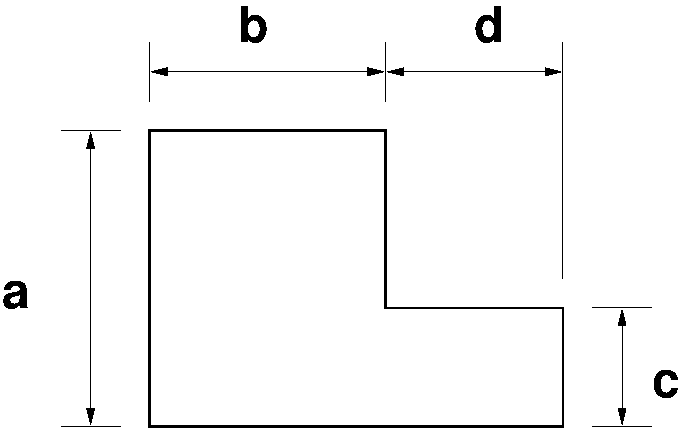
\includegraphics[width=0.6\textwidth]{./figuras/L2d.pdf}
\caption{Figura geométrica composta por dois retângulos}
\label{fig:L2d}
\end{figure}

Ao se multiplicar todas as dimensões características de um figura geométrica por uma constante, ou seja, na figura \ref{fig:L2d}, multiplicar $a$ por esta constante, o perímetro varia linearmente com esta constante e a área varia com o seu quadrado. Escolhendo $a'=k\cdot a$, a área $A'$ e perímetro $P'$ desta nova figura geométrica têm o seguinte valor:

\[
P' = \frac{a'}{a}\cdot P = k\cdot P \qquad A' = \left(\frac{a'}{a}\right)^2\cdot A = k^2\cdot A
\]

As grandezas que permanecem constantes quando se muda a escala da figura geométrica são parâmetros adimensionais.

\subsection{Teorema de pitágoras}

\begin{figure}
  \centering
  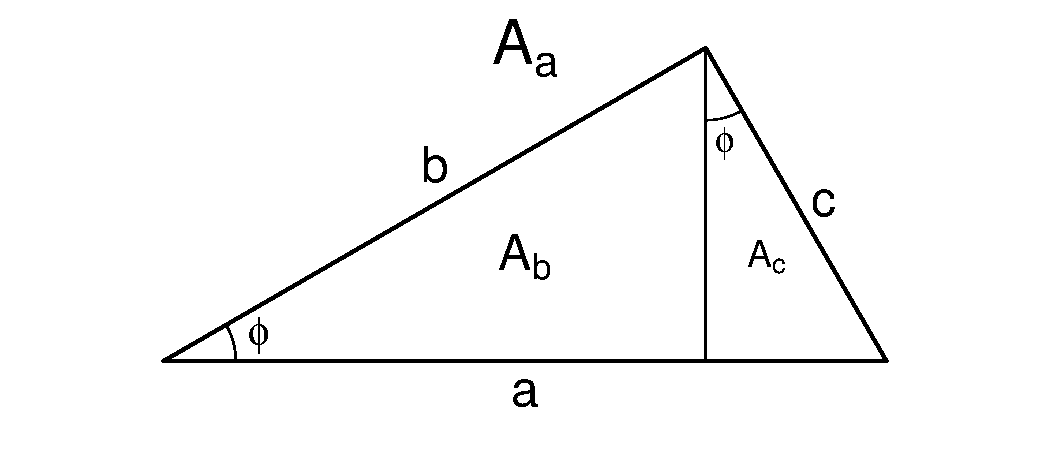
\includegraphics[width=0.9\textwidth]{./figuras/pitagoras}
  \caption{Teorema de Pitágoras}
  \label{fig:pit}
\end{figure}

Dois triângulos são semelhantes se dois ângulos são iguais. Se um dos ângulos é reto, o triângulo é chamado de de triângulo retângulo. Se a hipotenusa for escolhida como dimensão característica e o ângulo entre a hipotenusa e um cateto for denominado por $\phi$, a área deste triângulo é dada por uma relação do tipo
\[
A(h,\phi) = h^2\cdot f(\phi)
\]
A figura mostra como um triângulo retângulo pode ser dividido em dois triângulos retângulos semelhantes (mesmo ângulo $\phi$). Nesta subdivisão, 
\[
A_a a^2\cdot f(\phi) = A_b + A_c = b^2\cdot f(\phi) + c^2\cdot f(\phi)
\]

Dividindo por $f(\phi)$ chega-se ao teorema de Pitágoras:
\[
a^2 = b^2 + c^2
\]

Para concluir, esta demonstração do teorema de Pitágoras é resultado do fato de que a área de um triângulo é o produto entre hipotenusa ao quadrado e uma função do ângulo de um dos vértices, que não muda com a escala.


\subsection{Floco de Koch}

As relações anteriores contnuam válidas no caso de figuras geométricas mais ``exóticas''. A figura \ref{fig:koch} mostra um floco de Koch

\begin{figure}
\centering
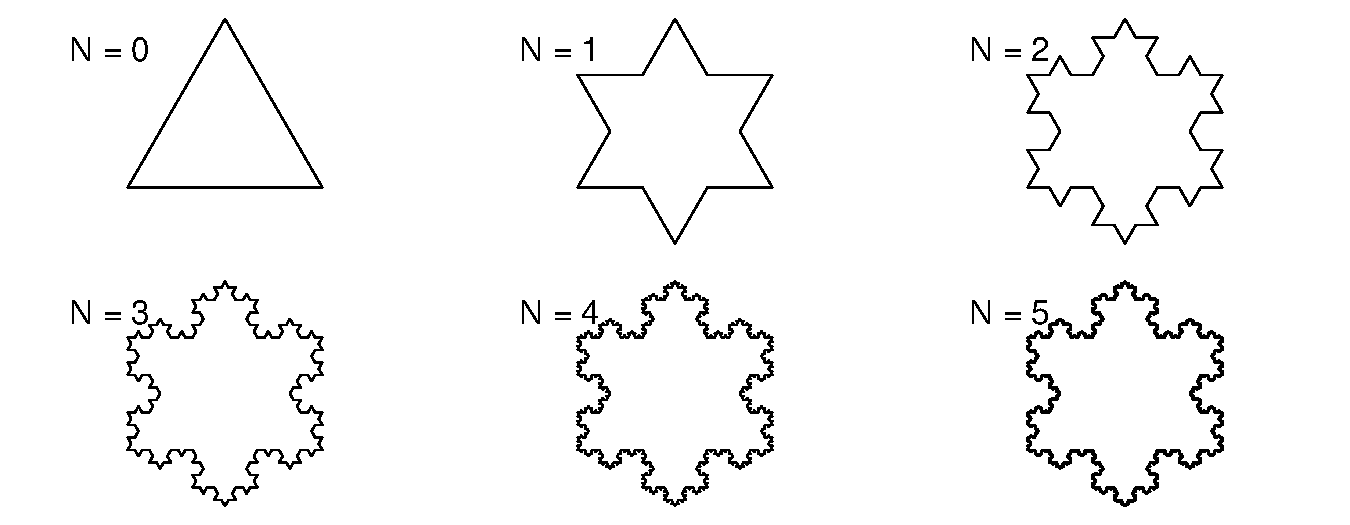
\includegraphics[width=\textwidth]{./figuras/koch.pdf}
\caption{Desenvolvimento do floco de Koch.}
\label{fig:koch}
\end{figure}

A área e perímetro do floco de Koch dependem da dimensão básica $L$ (lado do triângulo original) e o número de vezes $N$ que o floco é refinado. A área e o perímetro é dado por:
\[
\frac{A}{L^2} = \frac{\sqrt{3}}{20} \cdot \left[8 - 3\left(\frac{4}{9}\right)^N\right] \qrq \frac{P}{L} = 3\cdot\left(\frac{4}{3}\right)^N
\]
É interessante observar que no limite $N\lra\infty$ a área chega a um limite finito mas o mesmo não ocorre com o perímetro que sempre aumenta:

\[
\lim_{N\lra\infty} \frac{A}{L^2} = \frac{2}{5}\sqrt{3} \qquad\qquad \lim_{N\lra\infty}\frac{P}{L} = \infty
\]

Mas mesmo neste caso as regras dimensionais envolvendo a área e o perímetro continuam valendo se $N$ for fixado. Por outro lado se $N$ pode variar as relações anteriores indicam que aproximações são possívei em algum caso. Se o fenômeno em questão depender da área, basta escolher $N$ grande o suficiente. Já se depender do perímetro talvez seja necessário especificar $N$.

Este tipo de geometria pode parecer uma curiosidade matemática mas a natureza está repleta de coisas deste tipo. Qual o comprimento da costa do Brasil? Richardson (o mesmo da cascata de energia da turbulência, meteorologia computacional, etc) tentou determinar o comprimento da costa do Reino Unido e chegou em relações como a anterior. Qual a fronteira de uma nuvem? Em uma camada limite turbulenta, qual a geometria que separa o escoamento externo potencial do escoamento turbulento?

O floco de Koch também apresenta uma outra característica interessante e importante: auto-semelhança. A figura \ref{fig:koch-self} mostra vistas explodidas de uma seção do floco de Koch. Repare que os padrões se repetem em diferentes escalas. A auto-semelhança é observada em escalas intermediárias. Nas maiores escalas (muito maiores que o floco) ela deixa de ser observada. Nas menores escalas chegamos à resolução da figura e a auto-semelhança se perde. 

\begin{figure}
\centering
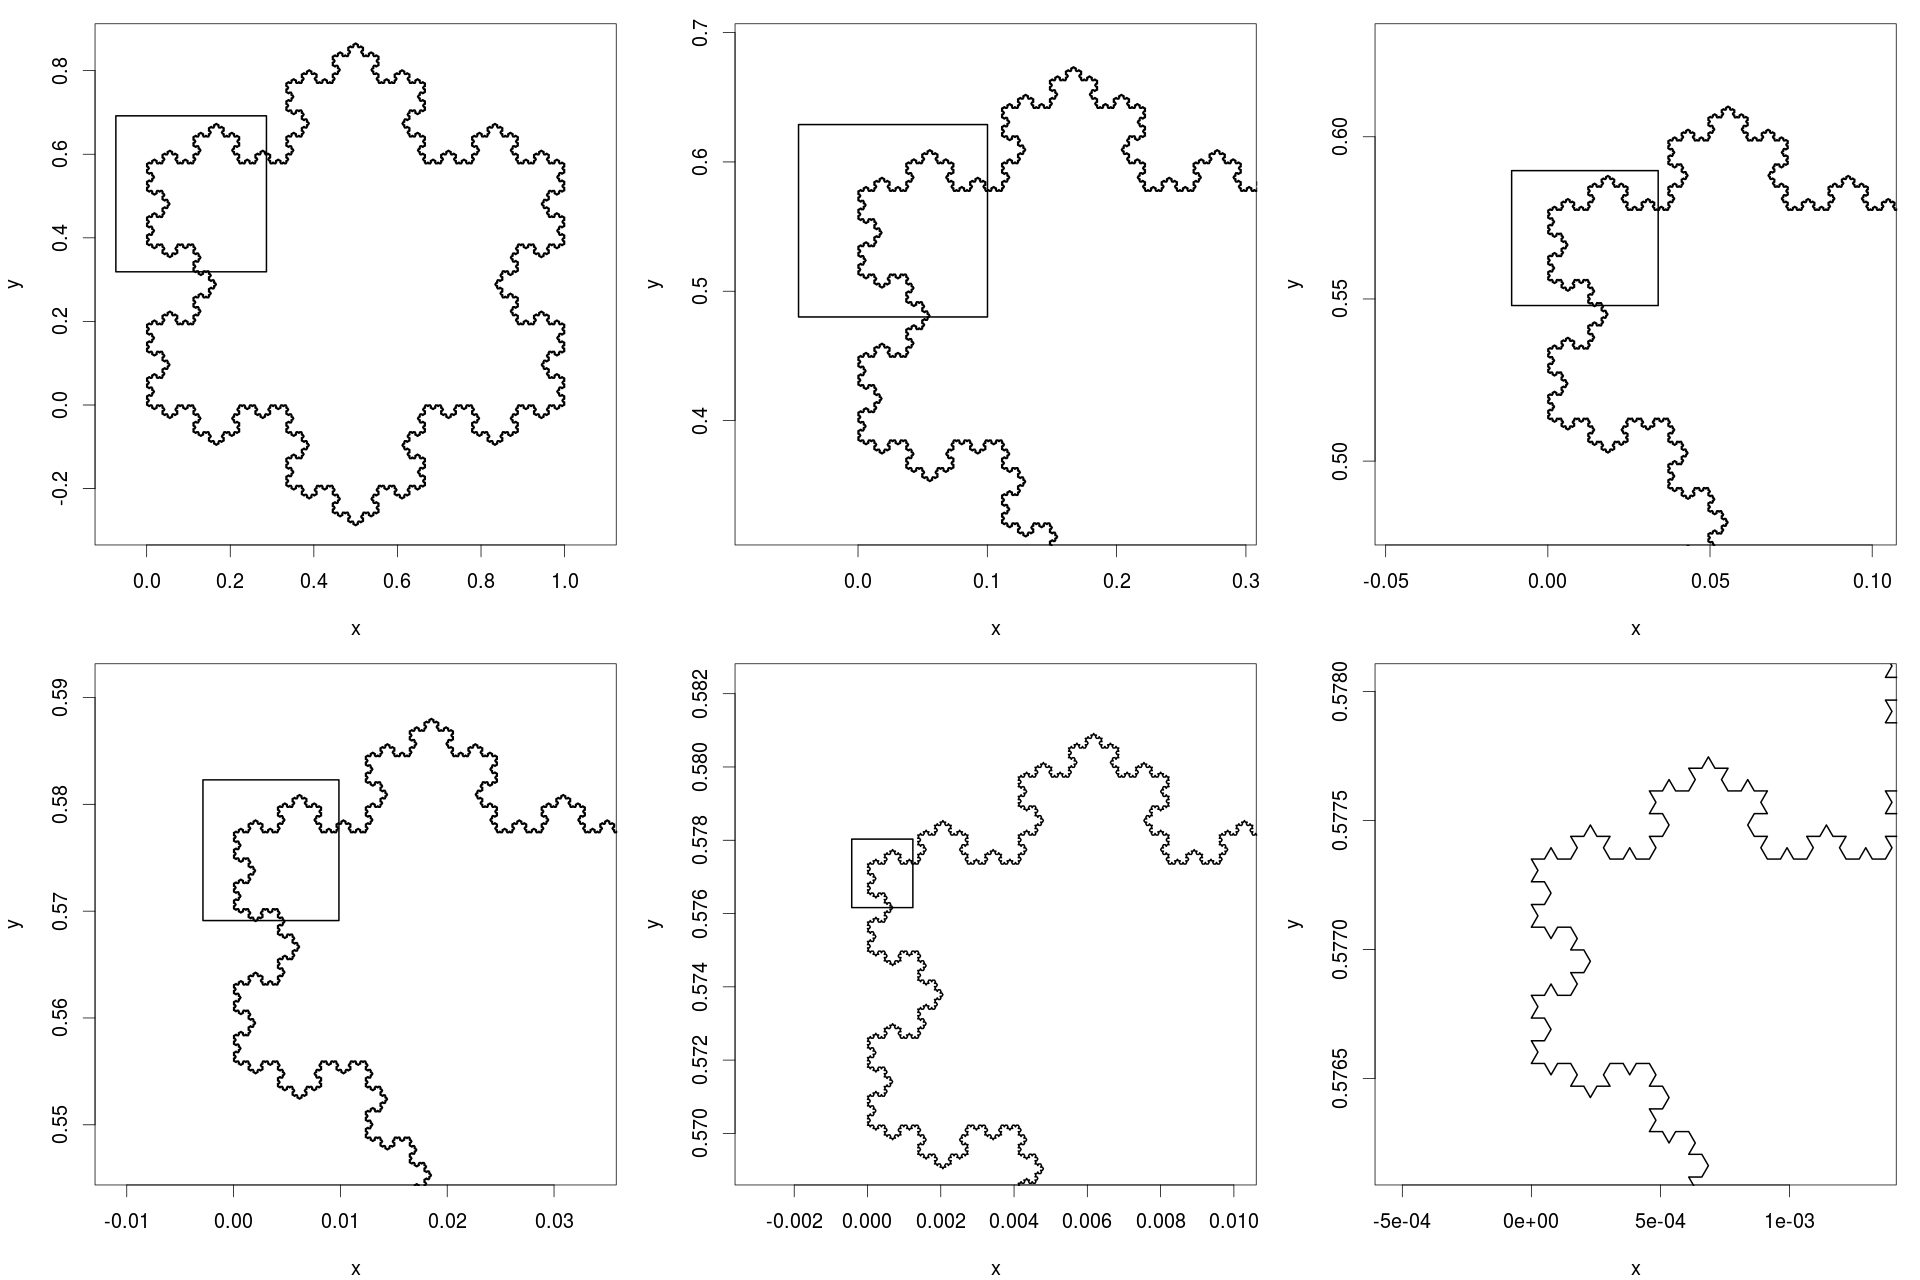
\includegraphics[width=1\textwidth]{./figuras/koch-self.png}
\caption{Auto-semelhança no floco de Koch.}
\label{fig:koch-self}
\end{figure}


O fenômeno da auto-semelhança não está restrita a geometrias exotéricas e fenômenos complexos. Sempre que leis de potência existirem, será observado auto-semelhança, como se vê na figura \ref{fig:power-law} onde a lei de potência 
\[
y = x^\frac{5}{2}
\]
é observada em diferentes escalas. Visualmente nada muda.

\begin{figure}
\centering
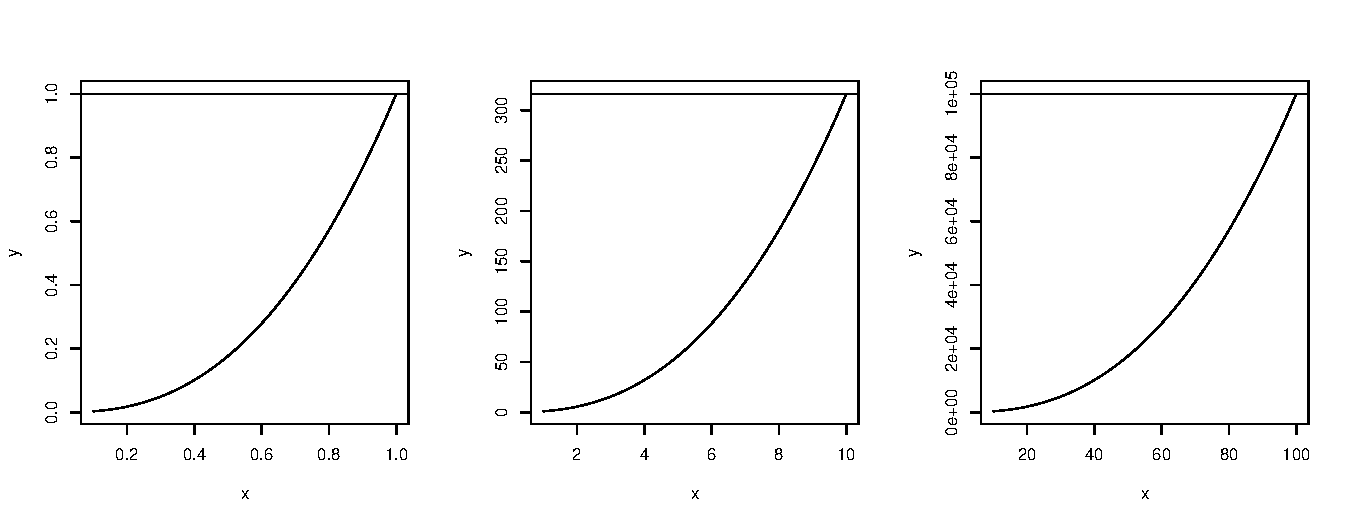
\includegraphics[width=\textwidth]{./figuras/power.pdf}
\caption{Auto-semelhança em leis de potência. A curva $y = x^{5/2}$ em diferentes escalas.}
\label{fig:power-law}
\end{figure}


\section{Equações diferenciais}
Boa parte do que se faz em ciência e tecnologia envolve fenômenos cujas equações básicas são conhecidas mesmo que se saiba pouco sobre o fenômeno em si. Tomemos como exemplo o escoamento de um fluido Newtoniano incompressível ao redor de um cilindro de grande comprimento. As equações básicas, equações de Navier-Stokes são conhecidas a quase 2 séculos mas este continua sendo um problema onde ocorre muita pesquisa, com muitos artigos em revistas científicas e pesquisadores ao redor do mundo empenhando grandes esforços neste problema aparentemente simples. Esta é uma situação comum em ciência. 

O fato de se conhecer os princípios básicos e as respectivas equações não quer dizer que o problema está resolvido. Mas é importante lembrar que estas equações continuam válidas mesmo que alguns detalhes do problema sejam nebulosos. Nesta seção, alguns problemas (modelos) serão analisados a partir de suas equações básicas.

\subsection{Pêndulo simples}

\begin{figure}
\centering
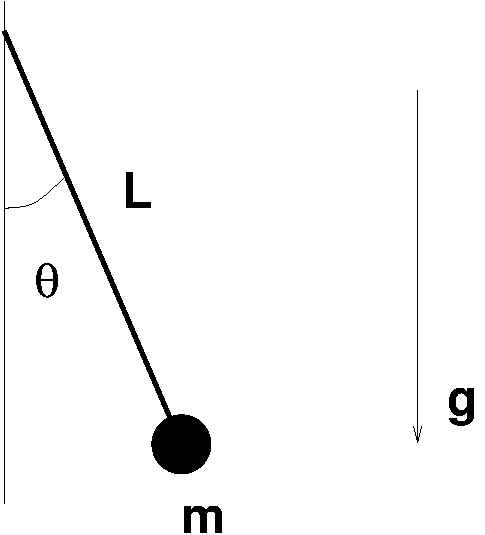
\includegraphics[width=0.4\textwidth]{./figuras/pendulo.pdf}
\vspace{0.5cm}
\caption{Pêndulo simples}
\label{fig:pendulo}
\end{figure}

O pêndulo simples é um dos problemas mais conhecidos na física básica. A figura \ref{fig:pendulo} mostra um diagrama esquemático do pêndulo simples. A palavra ``simples'' deve ser enfatizada. Este problema introdutório em cursos de físicas é uma idealização do problema real. Nesta idealização, os únicos parâmetros importantes são a massa do pêndulo, que neste modelo idealizado some, a aceleração da gravidade, que é constante, o comprimento do pêndulo e o ângulo inicial em que se solta o pêndulo. Nesta idealização, a dimensão da massa é desprezada e a única caractérística do fio é o seu comprimento que é constante. Efeitos como resitência do ar, elasticidade do fio, rotação da terra são desprezados. Se levados em conta, o problema é consideravelmente mais complexo. 

\subsubsection{O que se pode desprezar}
Mas não é tudo, outros fatores influenciam este problema como, por exemplo, a variação de $\textbf{g}$ com a posição. No limite, até a dinâmica dos átomos do ar e a radiação solar incidente interferem. Levando em conta tudo este problema não seria resolvido. Neste sentido, o mais importante é saber o que ignorar. Apenas os efeitos com as escalas corretas. Imaginemos que este pêndulo é uma esfera de aço com 1 cm de diâmetro. Se esta esfera refletir toda a luz incidente, a razão entre a força gerada pela pressão da luz do sol na terra e a força da gravidade vale (ordem de grandeza):
\[
\frac{F_{sol}}{F_{grav}} \approx \frac{W''}{\rho D g c} \approx 5\times 10^{-9}
\]
onde $W''=1360\:W/m^2$ é o fluxo de radiação solar. Com valores baixos como este, á fácil desprezar o efeito da radiação solar. 

Por outro lado, se o pêndulo tiver velocidade típica da esfera for de 1 m/s e estiver no ar, a razão entre a força peso e a força de arrasto aerodinâmica vale:
\[
\frac{F_{aero}}{F_{grav}} = \frac{3\cdot C_D \rho_a V^2}{32\cdot\rho D g} \approx 0,02\%
\]

Este valor de 0,02\% é pequeno mas seu efeito acumulado pode ser considerável (pêndulos param) e dependendo do que se deseja, deve ser incluido. No entanto, é importante observar que, por este valor ser pequeno, um modelo simples com incerteza alta para a força de arrasto geralmente é suficiente para a maioria dos problemas. Caso contrário teria que se resolver o problema do escoamento ao redor da esfera, o que, como será visto adiante, não é um problema simples.

\subsubsection{Modelo matemático simples}
Com todas as simplificações anteriores, chega-se à equação do pêndulo simples:

\[
m\cdot L^2\cdot\frac{d^2\theta}{dt^2} + m\cdot g\cdot L\cdot \sin\theta = 0
\]
com as seguintes condições de contorno:
\[
t = 0 \qrq \theta=\theta_0, \quad\frac{d\theta}{dt} = 0
\]

Esta equação pode ser reescrita como:
\[
\frac{L}{g}\frac{d^2\theta}{dt^2} + \sin\theta = 0 
\]
Definindo 
\[
t_* = \frac{t}{t_0}\qrq \quad\text{onde}\quad t_0 = \sqrt{\frac{L}{g}}
\]
chega-se à equação adimensional
\[
\frac{d^2\theta}{dt_*^2} + \sin\theta = 0 
\]

Agora, sabendo $\theta_0$ (condição de contorno inicial) resolvendo esta equação, está se resolvendo qualquer pêndulo simples. Quando $\theta_0$ é pequeno, $\sin\theta_0\approx\theta_0$ e a equação diferencial é linearizada. Sua solução é simples e o período do pêndulo vale:
\[
T = 2\pi\sqrt{\frac{L}{g}}
\]
Partindo desta solução aproximada pode-se obter uma expressão para o problema não linear utilizando métodos assintóticos:
\[
T = 2\pi\sqrt{\frac{L}{g}}\cdot\varphi(\theta_0) = 2\pi \sqrt{\frac{L}{g}} \cdot\left[\varphi(0) + \theta_0\cdot\varphi'(0) +
\frac{1}{2}\theta_0^2\cdot\varphi'' + \ldots\right]
\]
o que se observa neste problema simples é que a formulação do problema simplificado (idealizado) exige a desprezar diferentes fenômenos físicos. Para tanto é necessário achar estimativas, mesmo que grosseiras, das diferentes influências. Uma vez que se simplificou o problema, pode-se fazer mais, utilizando análise dimensional, o que consiste basicamente em reescalar o problema. Neste ponto maiores simplificações são, algumas vezes, possíveis.

Uma outra maneira se enxergar este processo (análise dimensional) é considerar que pode-se escolher um outro sistema de unidades onde os coeficientes (neste caso $\sqrt{L/g}$) valem 1.

\subsection{Difusão de calor}
\subsubsection{Problema 3D}
Neste caso, o problema é modelado por uma equação diferencial parcial. Vale ressaltar que para se chegar a esta equação diferencial, o problema já foi simplificado. O problema da difusão de calor linear é modelado pela seguinte equação diferencial:
\[
\frac{\partial u}{\partial t} = \alpha\nabla^2 u
\]
onde $u$ é a temperatura e $\alpha$ é o coeficiente de difusão de calor do material. Além disso, ainda faltam as condições de contorno. Quando o domínio é um cubo de lado $L$ formado pelas faces $x=0,L$m $y=0,L$ e $z=0,L$ e as condições de contorno forem $u=0$ na face $x=0$, $u=u_0$ e nas demais o fluxo de calor é nulo, ou seja, a derivada da temperatura em relação à normal da face é zero. A condição inicial é $u=0$. O objetivo deste problema é obter $u(x,y,z,t)$ para $t>0$:
\[
u = f(u_0, L, \alpha, x, y, z, t)
\]
A equação fornece uma escala de dimensão $L$ e escala de temperatura $u_0$. Estas escalas permitem definir novos parâmetros que na região de interesse possuem valores da ordem de 1: $x_* = x\cdot L$, $y_* = y\cdot L$, $z_* = z\cdot L$, e $u_* = u\cdot u_0$. Dentro do cubo, tanto as coordenadas $(x_*, y_*, z_*)$ quanto a temperatura $u_*$  possuem valores entre 0 e 1. Substituindo estas relações na equação diferencial temos:
\[
\frac{\pd u_*}{\pd t} = \frac{\alpha}{L^2}\left(\frac{\pd^2 u_*}{\pd x_*^2} + \frac{\pd^2 u_*}{\pd y_*^2} + \frac{\pd^2 u_*}{\pd z_*^2} \right) = \frac{\alpha}{L^2} \nabla_* u_*
\]
Esta equação sugere uma escala de tempo: $t = t_*\cdot t_0 = t_* \cdot \frac{L^2}{\alpha}$. Substituindo esta relação na equação anterior chega-se à seguinte relação:
\[
\frac{\pd u_*}{\pd t_*} =\nabla_* u_*
\]
As condições de contorno são $u_*=0$ em $x_*=0$, $u_*=1$ em $x_*=1$ e nas demais faces o fluxo é zero: $\pd u_*/\pd y_* = 0$ em $z_*=0,1$ e $\pd u_*/\pd z_* = 0$ em em $y_*=0,1$.


As condições de contorno também se simplificam: $u_*=0$ em $x_*=0$, $y_*=0$, $z_*=0$, $y_*=1$, $z_*=1$ e $u_* = 1$ em $x_* = 1$. 

A solução deste novo problema é:
\[
u = u_0 \cdot \varphi(t_*, x_*, y_*, z_*) = u_0\cdot\varphi\left(\frac{t\alpha}{L^2}, \frac{x}{L}, 
 \frac{y}{L} , \frac{z}{L}\right)
\]
O problema original tinha 7 parâmetros e foi reduzido para 4, o que é um ganho substancial. Novamente, para este tipo de geometria e este tipo de condição de contorno, a solução deste problema adimensional vale para quaisquer valores de $L$, $\alpha$ e $u_0$. Outro aspecto interessante é que no domínio/tempo de interesse, todos os parâmetros são da ordem um, $\mathcal{O}(1)$.

\subsubsection{Uma barra fina e comprida}

Modificando o problema de modo que o domínio é um paralelepípedo com lados $L_x=L$, $L_y$ e $L_z$, onde $L \gg L_x$ e $L \gg L_y$, as variações da temperatura nas direções $y$ e $z$ para $x$ constante são desprezíveis e portanto a equação diferencial pode ser simplificada de modo que 
\[
u(x, y, z, t) = u(x, t)
\]
e portanto

\[
\frac{\pd u}{\pd t} = \alpha \frac{\pd^2 u}{\pd x^2}
\]
Como na subseção anterior, chega-se a uma equação adimensional. Repetindo o procedimento da seção anterior, chega-se à seguinte equação adimensional:
\[
\frac{\pd u_*}{\pd t_*} = \frac{\pd^2 u_*}{\pd x_*^2} \qrq u = u_0\cdot\varphi\left(\frac{t\alpha}{L^2}, \frac{x}{L}\right)
\]
A solução deste problema com $t\lra\infty$ é a velha distribuição linear de temperatura:
\[
u(x,\infty) \lra \frac{x}{L}\cdot u_0
\]
Mas nos outros instantes de tempo é necessário resolver a equação acima. Outras simplificações são possíveis quando $L$ é muito grande ou quando $t$ é muito pequeno.

\subsubsection{Auto-semelhança: barra infinita}
O que acontece se a barra for muito comprida (ou o logo no começo)? Neste caso, não existe uma escala de comprimento pré-definida. Assim esta escala deve sair do próprio problema. Ou seja, se $L\lra\infty$, para que o tempo adimensional seja constante:
\[
\frac{t\alpha}{L^2} = cte \qrq L = \sqrt{t\alpha} \qrq \eta = \frac{x}{L} = \frac{x}{\sqrt{\alpha t}} \qrq \frac{u}{u_0} = f(\eta)
\]
Usando esta escala na equação diferencial parcial, chega-se à seguinte equação diferencial \emph{ordinária}:
\[
f''(\eta) + \frac{\eta}{2} f'(\eta) = 0
\]
com condições de contorno
\[
f(0) = 0 \qquad\qquad \lim_{\eta\lra\infty} f(\eta) = 1
\]
Com esta mudança de variáveis, transformou-se uma equação diferencial parcial em uma equação diferencial ordinária, algo que é significativo. Neste caso, a solução analítica desta equação é simples:
\[
f(\eta) = \mathrm{erf}\left(\frac{\eta}{2}\right)
\]
onde $\mathrm{erf}$ é a função erro.

\section{Escoamento incompressível ao redor de uma esfera}


Os examplos anteriores usaram modelos simples e/ou lineares para mostrar como as principais escalas de um problema permitem simplificar equações diferenciais. Nesta seção será analisado o escoamento ao redor de uma esfera. Admitindo um fluido newtoniano incompressível, chega-se às equações de Navier-Stokes:

\begin{equation}
\frac{\pd\p{u}}{\pd t} + \p{u}\cdot\nabla\p{u} = -\frac{1}{\rho}\nabla p + \nu\nabla^2\p{u} \qquad\qquad \nabla\cdot\p{u} = 0
\label{eq:ns}
\end{equation}
onde $\p{u}$ é o vetor velocidade, $p$ é o campo de pressões, $\nu$ é a viscosidade cinemática e $\rho$ é a densidade do fluido. O problema do escoamento ao redor de uma esfera em um ambiente grande apresenta as seguintes condições de contorno:
\[
 r\lra\infty \quad \p{u}\lra U_0\p{\hat{i}} \qquad\qquad r=\frac{D}{2}\quad \p{u} = \p{0}
\]
a segunda condição anterior corresponde à aderência do fluido na parede da esfera. Estas condições de contorno fornecem uma escala para a velocidade $U_0$ e uma escala para a dimensão $D$ (o diâmetro da esfera). Seguindo o mesmo procedimento adotado para o problema de difusão, obtém-se os seguintes parâmetros para o problema:

\[
\begin{aligned}
&x_* = \frac{x}{D}, \quad y_* = \frac{y}{D}, \quad z_* = \frac{z}{D}\\
&\p{u}_* = \frac{\p{u}}{U_0}, \quad p_* = \frac{p}{P_0}, \quad t_* = \frac{t}{t_0} = \frac{tU_0}{D} \\
\end{aligned}
\]
Observe que o parâmetro $P_0$ ainda é desconhecido e será analisado mais adiante. Antes, porém, é interessante notar que não existe uma equação para a pressão e ela não aparece nas condições de contorno. Na verdade, a pressão ela aparece como resultado das equações de Navier-Stokes e seu valor é tal que a equação da continuidade ($\nabla\cdot\p{u}=0$) é satisfeita. Usando as escalas corretas os parâmetros anteriores possuem valores com ordem de grandeza $\mathcal{O}(1)$. Isto pode parecer estranho a primeira vista já que o domínio se estendo ao infinito. No entanto as coisas mais relevantes acontecem perto da esfera. É neste sentido que $x_*, y_*, z_* \sim 1$. Um argumento semelhante pode ser utilizado para o tempo $t_*$. É lógico que o escoamento pode durar um intervalo de tempo grande (uma bola pode ficar durante dias dentro de um túnel de vento) mas o tempo que leva para uma partícula passar por perto da esfera corresponde a  $t_*\sim 1$. 

Com estes novos parâmetros, chega-se às equações de Navier-Stokes adimensionais:

\begin{equation}
\frac{\pd\p{u}_*}{\pd t_*} + \p{u}_*\cdot\nabla_*\p{u_*} = -\frac{P_0}{\rho U_0^2}\nabla_* p_* + \frac{1}{Re}\nabla_*^2\p{u}_* \qquad \nabla_*\cdot\p{u}_* = 0
\label{eq:ans}
\end{equation}
nestas equações, $Re = \frac{U_0 D}{\nu}$ é o número de Reynolds e 
\[
\nabla_* = \frac{\pd}{\pd x_*} \p{\hat{i}} + \frac{\pd}{\pd y_*} \p{\hat{j}} + \frac{\pd}{\pd z_*} \p{\hat{k}}
\]
e as condições de contorno são:
\[
 r_*\lra\infty \quad \p{u}_*\lra \p{\hat{i}} \qquad\qquad r_*=\frac{1}{2}, \p{u}_* = \p{0}
\]

Como se observou para o pêndulo simples e a difusão de calor, introduzir as escalas principais do problema reduz o trabalho significativamente se originalmente
\[
u = f(t, x, y, z, U_0, D, \nu, \rho)
\]
Com esta análise dimensional, o problema se reduziu a 
\[
u = U_0 \varphi\left(\frac{t U_0}{D}, \frac{x}{D}, \frac{y}{D}, \frac{z}{D}, \frac{U_0 D}{\nu}\right)
\]

Se antes, além do tempo e coordenadas,  eram  necessários resolver o problema para quatro parâmetros independentes ($U_0$, $D$, $\nu$ e $\rho$), agora, apenas o número de Reynolds é necessário. A economia de esforços é considerável, assim como a liberdade que se ganha: experimentos podem ser realizados em diferentes fluidos se $Re$ for o mesmo.

Este resultado ó obtido na análise dimensional tradicional. No entanto é interessante lembrar que nesta formulação, cada termo $u_*$ tem ordem de grandeza 1 por construção e aparecem dentro de derivadas. Dependendo das circunstâncias, estimativas relativas de cada termo desta equação podem ser feitas de modo a desprezar alguns termos e simplificar o problema.

\subsection{Equações de Euler - $Re\lra\infty$}

Uma aproximação de \ref{eq:ans} que salta à vista é o limite 
\[
Re \lra\infty
\]
Se admitirmos que o escoamento está em regime permanente (RP), $\pd/\pd t = 0$, obtém-se as equações de Euler:

\begin{equation}
\p{u}_*\cdot\nabla_*\p{u_*} = -\frac{P_0}{\rho U_0^2}\nabla_* p_* %\qqrq P_0\sim\rho U_0^2
\label{eq:euler}
\end{equation}
por construção, o lado esquerdo desta equação tem ordem de grandeza 1. Para que o gradiente de pressão tenha, também, ordem de grandeza 1, é basta definir  
\[
P_0 = \rho U_0^2
\]

A equação de Euler ainda possue o termo convectivo não linear mas já não é uma equação de segunda ordem. Isto tem consequências, principalmente perto da parede pois nas equações de Euler, a velocidade junto a parede não é nula. Mas longe da parede as equações de Euler podem ser representativas, principalmente se não houver separação.

\subsection{Equação de Stokes}
Um outro limite é quando $Re\lra 0$. Neste caso não faz sentido empregar $P_0 = \rho U_0^2$ que foi obtido admitindo $Re$ grande. Novamente, considerando o escoamento em regime permanente e multiplicando ambos os lados da equação por $Re$, 
\[
Re\left(\p{u}_*\cdot\nabla_*\p{u_*}\right) = -Re\frac{P_0}{\rho U_0^2}\nabla_* p_* + \nabla_*^2\p{u}_* \qquad\qquad \nabla_*\p{u}_* = 0
\]
por construção, o termo convectivo tem ordem 1 e  vai para zero. Infelizmente não se pode simplesmente desprezar o termo da pressão. Fazendo $Re$ tender a zero mantendo $D$, $\rho$ e $\nu$ fixos, o denominador $\rho U_0^2$ vai para zero mais rapidamente que $Re$ que está no numerador e portanto este termo não pode ser desprezado. No entanto uma nova escala para pressão surge. Se
\[
Re\cdot\frac{P_0}{\rho U_0^2} = 1 \qrq P_0 = \frac{\mu}{U_0}{D}
\]

Com esta nova escala para a pressão, as equações de Stokes tomam a forma final
\begin{equation}
\nabla_* p_* + \nabla_*^2\p{u}_* = 0 \qquad\qquad \nabla_*\cdot\p{u}_* = 0
\label{eq:stokes}
\end{equation}

Em geral, em um escoamento incompressível, a força de arrasto em um corpo é a soma de duas contribuições: a integral da pressão e a integral das tensões de cisalhamento na superfície do corpo. No caso da equação de Stokes, as forças devido à pressão apresentam a seguinte ordem de grandeza:
\[
F_P \sim P_0 \cdot A \approx P_0 \cdot D^2 =\mu U_0 D
\]
A tensão de cisalhamente pode ser estimada como $\tau \sim \mu U_0 / D$ de modo que 
\[
F_V \sim \tau \cdot A \approx \mu U_0 D
\]
Assim, a força de arrasto deve valer:
\[
F_D = k \cdot \mu U_0 D
\]
onde $k$ é uma constante que depende da geometria do corpo. Stokes obteve a seguinte relação para a força de arrasto em uma esfera:
\begin{equation}
F_D = 6\pi\mu U_0 D
\label{eq:cdstokes}
\end{equation}

É interessante observar que a equação de stokes tem dois termos, um contendo a pressão o outro a velocidade de modo que existe um equilíbrio entre estes dois termos. Se um sobe localmente, o outro terá que subir imediatamente para manter o equilíbrio. Neste sentido o fato de que as estimativas $F_P$ e $F_V$ têm a mesma forma é esperado.

\subsection{E Stokes para um cilindro infinito?}
A princípio, a análise que foi feita para se obter a equação de Stokes para uma esfera poderia ser repetida para qualquer corpo. Não foi feita nenhuma hipótese quanto a geometria do corpo além de se impor uma escala dimensional. Entretanto quando tenta fazer a mesma análise para um cilindro muito longo, a equação de Stokes não tem solução. Este fato é conhecido como o \emph{Paradoxo de Stokes} \cite{Birkhoff60}. O melhor que se pode fazer é linearizar o termo convectivo, obtendo-se a seguinte equação:

\[
Re\:\hat{\p{i}}\cdot\nabla_*\p{u_*} = -\nabla_* p_* + \nabla_*^2\p{u}_*
\]

\subsection{Velocidade variando ciclicamente}
Até este ponto, admitiu-se que o escoamento estava em regime permanente. Assim, a escala de tempo é produto do próprio escoamento e suas escalas de velocidade ($U_0$) e dimensão ($D$) com $t_0 = D/U_0$. No entanto, uma escala externa de tempo externa pode ser imposta se a velocidade ao longe valer
\[
U_\infty = U_0\cdot\left(1 + \epsilon_0\cdot\cos \omega_0 t\right)
\]
esta velocidade oscilante introduz uma nova escala de tempo $t_1 = 1/\omega_0$. Ao invés da escala de tempo $t_0 = D/U_0$ esta nova escala de tempo for utilizada para se definir a $t_*$. Com isso a equação de Navier-Stokes adimensional tem a seguinte forma:

\begin{equation}
\Omega\frac{\pd\p{u}_*}{\pd t_*} + \p{u}_*\cdot\nabla_*\p{u_*} = -\frac{P_0}{\rho U_0^2}\nabla_* p_* + \frac{1}{Re}\nabla_*^2\p{u}_*  \qquad \Omega = \frac{D\omega_0}{U_0}
\label{eq:nstemp}
\end{equation}

Além de $Re$, um novo parâmetro aparece: $\Omega$. Este novo parâmetro nada mais é que a razão entre as duas escalas de tempo do problema:
\[
\Omega = \frac{t_0}{t_1} = \frac{D\omega_0}{U_0}
\]

Se a velocidade ao longe for uma expressão do tipo 
\[
U_\infty = U_0\cdot\left(1 + \sum_{k=0}^{N-1}\epsilon_k\cdot\cos \omega_k t\right)
\]
novas escalas de tempo são introduzidas: $1/\omega_1, 1/\omega_2, \ldots, 1/\omega_{N-1}$. Cada escala de tempo $t_k = 1/\omega_k$ introduz um novo parâmetro adimensional $\Omega_k = t_0/t_{k+1} = D\omega_k/U_0$.

É interessante observar que se por um lado, um campo de velocidades variando ciclicamente com várias frequências parece algo exotérico, é isto o que acontece em um escoamento turbulento que tem um espectro contínuo que deve ser modelado. Além disso todas as três componentes de velocidade variam e estão correlacionadas entre si. Isto parece ser muito mais difícil de se simular experimentalmente (ou mesmo numericamente) mas na prática, se $Re$ for alto o suficiente, basta gerar um escoamento com escala integral correta que um espectro padrão (Von Karman por exemplo) surge.

\subsection{Esfera em uma base elástica}
Esta é uma situação comum onde a esfera (ou outro corpo) não está fixo mas pode se mover em torno de um ponto. Este caso introduz uma nova equação. Além da dinâmica do fluido externo ao corpo, é necessário modelar a dinâmica do próprio corpo. O modelo mais simples consiste em um sistema massa-mola-amortecedor de 1 graus de liberdade. Se o corpo tem uma massa $m$ e a base tem rigidez $k$, a frequência natural introduz uma outra escala de tempo:
\[
\frac{1}{t_2}  = \omega_N = \sqrt{\frac{k}{m}} \qqrq t_* = \frac{t}{t_0} = t\cdot \frac{U_0}{D}
\]

A razão entre as duas escalas de tempo é um novo parâmetro adimensional conhecido como velocidade reduzida:
\[
V_R = \frac{t_2}{t_0} = \frac{U_0}{\omega_N\cdot D} \quad \text{Velocidade reduzida}
\]

 Na equação de Navier-Stokes pode-se escolher $t_0$ ou $t_2$ como escala de tempo. Escolhendo $t_0$, obtém-se a equação adimensional original (eq. \ref{eq:ns}):
\[
\frac{\pd\p{u}_*}{\pd t_*} + \p{u}_*\cdot\nabla_*\p{u_*} = -\frac{P_0}{\rho U_0^2}\nabla_* p_* + \frac{1}{Re}\nabla_*^2\p{u}_* 
\]

Ainda falta analisar a equação do oscilador:
\[
y''(t) + 2\zeta\omega_Ny'(t) + \omega_N^2y(t) = \frac{F(y, y', t)}{m}
\]
onde $\zeta$ é a razão de amortecimento crítico e $F$ é uma função que fornece as forças do fluido agindo na massa. Usando \emph{as mesmas escalas de comprimento ($D$) e de tempo $t_0$} esta equação pode ser reescrita como
\[
\frac{d^2y_*}{dt_*^2} + 2\frac{\zeta}{V_R} \frac{dy_*}{dt_*} + \frac{1}{V_R^2} y_* = \frac{\rho D^3}{m} \cdot \varphi\left(t_*, y_*, y'_*\right)
\]
Nesta equação, além da velocidade reduzida ($V_R$) aparece um outro adimensional $\rho D^3/m$ que é a razão entre massa de fluido deslocado pela esfera e a massa da esfera. A força, por sua vez, foi obtida a partir de uma função adimensional $\varphi$ multiplicada por uma força de referência - a pressão dinâmica vezes a área: $\rho U_0^2 \times D^2 \varphi(t_*, y_*, y'_*)$.

Naturalmente, poderia-se adimensionalizar a equação de Navier-Stokes utilizando a escala de tempo do oscilador $t_2$. Neste caso a equação de Navier-Stokes adimensional fica diferente 

\[
\frac{1}{V_R}\frac{\pd\p{u}_*}{\pd t_*} + \p{u}_*\cdot\nabla_*\p{u_*} = -\frac{P_0}{\rho U_0^2}\nabla_* p_* + \frac{1}{Re}\nabla_*^2\p{u}_* 
\]
Esta equação é muito parecida com a equação obtida para o caso com a velocidade ao longe variando ciclicamente ($V_R$ é muito parecido com $1/\Omega$). 

A equação do oscilador toma a seguinte forma:
\[
\frac{d^2y_*}{dt_*^2} + 2\zeta\frac{dy_*}{dt_*} + y_* = \frac{\rho D^3}{m} \cdot V_R^2 \cdot \varphi_1\left(t_*, y_*, y'_*\right)
\]
Como era de se esperar os mesmos parâmetros adimensionais $V_R$, $\rho D^3/m$ e $Re$ aparecem.

\subsection{Camada Limite quando $Re\lra\infty$ e solução de Blasius para a placa plana}

As equações de Euler foram obtidas desprezando o termo difusivo (viscoso) quando $Re\lra\infty$. Como já foi visto,  sabe-se que isso introduz uma dificuldade, conhecida como o paradoxo D'Alembert \cite{Birkhoff60}. Este paradoxo só foi resolvido em 1904 quando L. Prantl introduziu  o conceito de camada limite \cite{Birkhoff60}. O problema é que utilizar a escala de comprimento $D$ para se estimar o termo difusivo é inconsistente com a realidade: a mudança da velocidade de zero (na parede) até um valor alto da ordem de $U_0$ ocorre em uma região muito pequena próxima à parede com dimensões características $\delta$, onde $\delta \ll D$, e portanto o  gradiente de velocidade é elevado e o termo difusivo não pode ser simplesmente desprezado (nesta região próxima à parede). A espessura da camada limite $\delta$ é uma outra escala do problema. Esta nova escala de comprimento é de natureza distinta da escala original $D$ pois não é algo se enxerga imediatamente mas sim produto do próprio escoamento. Neste contexto,  não é coincidência, então, que levou tanto tempo para alguém propor a teoria da camada limite. Muito do que se discutiu até este momento pode ser aplicado como um algorítmo mas introduzindo um pouco de física pode-se ir muito além.

\subsubsection{Estimativa da espessura da camada limite}
As equações diferenciais já analisadas tinham variáveis dependentes (como velocidade, temperatura, etc) e variáveis independentes (coordenadas no espaço e tempo) e parâmetros (viscosidade, etc). Assim, o procedimento adotado foi escolher escalas adequadas de modo a construir parâmetros adimensionais (variáveis com subíndice ``$*$'') que tivessem ordem de grandeza 1 na região de interesse. Um outro jeito de enxergar isso, é mudar o sistema de unidades de modo que as grandezas, neste novo sistema tenham valores própximos de 1. No caso do escoamento ao redor da esfera, isto consiste em utilzar um sistema de unidades onde o diâmetro da esfera tem valor numérico igual a 1 assim como a velocidade ao longe. Isto é o que se chama, tradicionalmente, de análise dimensional e será discutido mais adiante. 

A vantagem de se adotar estas escalas como referência (ou mudar o sistema de unidades) é que fica fácil comparar diretamente as ordens de grandeza de cada termo da equação que modela o fenômeno e desprezar  os termos pequenos. Isto pode ser sedutor mas sem cuidado (outro jeito de dizer ``sem conhecer os fenômenos físicos relevantes''), pode-se chegar a problemas como o paradoxo de Stokes ou o paradoxo D'Alembert. 

Mas por outro lado, conhecendo estas possíveis dificuldades novas escalas podem ser introduzidas de maneira apropriada. Em geral, o fato das variáveis dependentes e independentes tiverem, por construção valores de ordem 1, sugere uma outra abordagem. Como exemplo, seja a derivada no espaço da velocidade:
\[
\frac{\partial u}{\partial x} = \frac{U_0}{D}\frac{\partial u_*}{x_*} \sim \frac{U_0}{D}
\]
a última expressão reflete o fato de que a velocidade varia entre valores da ordem de $U_0$ e $0$ em regiões com ordem de grandeza $D$. Naturalmente, como já foi observado,  existem situações onde estas estimativas estão completamente fora como por exemplo na camada limite onde a mesma variação de velocidade (de zero a algo da ordem de $U_0$) ocorrerá em uma região muito menor (da ordem da espessura da camada limite $\delta$). Mas mesmo neste caso, nesta família de problemas, a razão $D/\delta\sim\gamma$ é mais ou menos constante. 

Voltando à equação de Navier-Stokes, estas estimativas podem ser empregadas diretamente:
\begin{equation}
\begin{matrix}
\frac{\pd\p{u}}{\pd t}& +& \p{u}\cdot\nabla\p{u}& = &-\frac{1}{\rho}\nabla p& +& \nu\nabla^2\p{u}\\
\bigO{\frac{U_0^2}{D}}& & \bigO{\frac{U_0^2}{D}} &  & \bigO{\frac{U_0^2}{D}}&  & \xcancel{\bigO{\nu\frac{U_0}{D^2}}} \\
 & & & & & & \bigO{\nu\frac{U_0}{\delta^2}}\\
\end{matrix}
\label{eq:ns-o}
\end{equation}
onde a estimativa já obtida $P\sim \rho U_0^2$ foi utilizada. A primeira reação é, se $Re$ for alto, desprezar o termo difusivo. Mas como sabemos que este termo é importante, pelo menos em uma região do escoamento, nesta região, este termo deve tem \emph{pelo menos a mesma ordem de grandeza que os outros termos da equação}. O problema não está na estimativa da variação da velocidade e sim na distância onde esta variação ocorre que foi chamada de $\delta$. É importante realçar que esta estimativa para o termo difusivo é apenas o pior caso. Fora da camada limite, este termo é desprezível o que quer dizer que \emph{a soma dos outros termos é nula}, apesar de que a estimativa da ordem de grandeza de cada termo seja $U_0^2/D$. Em um caso mais geral, a soma dos outros termos da equação poderiam cancelar em maior ou menor grau resultando em diferentes estimativas da ordem de grandeza deste termo.

Tendo isso em mente, pode-se chegar a uma estimativa da ordem de grandeza da espessura da camada limite:
\[
\frac{U_0^2}{D} \sim \nu\frac{U_0}{\delta^2}
\]
admitindo que não há cancelamento na soma dos outros termos da equação. Com esta hipótese, esta relação permite obter-se uma estimativa para a escala de comprimento da espessura da camada limite:
\begin{equation}
\frac{U_0^2}{D} \sim \nu\frac{U_0}{\delta^2} \qrq \frac{\delta}{D} \sim \sqrt{\frac{1}{Re}}
\label{eq:delta}
\end{equation}
Esta expressão é consistente com a solução de Blasius para a camada limite laminar \cite{Tritton88}.



\subsubsection{A camada limite na placa plana}

\begin{figure}
\centering
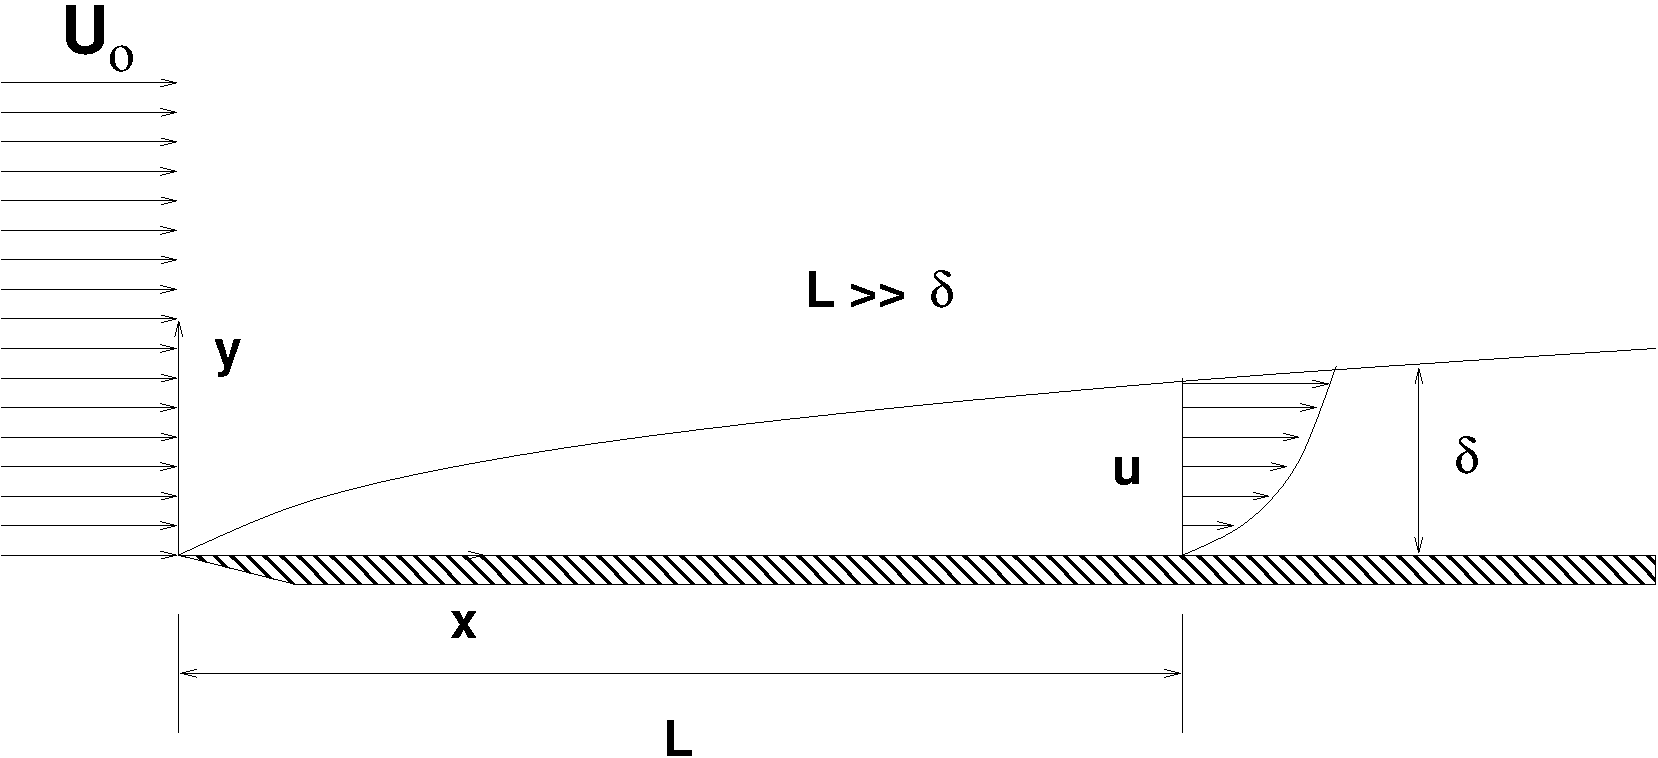
\includegraphics[width=0.85\textwidth]{./figuras/camada-limite.pdf}
\caption{Camada limite em uma placa plana}
\label{fig:blayer}
\end{figure}

Este tipo de análise pode ser levada mais adiante. Um problema mais simples é o escoamento em uma placa plana que pode ser visto na figura \ref{fig:blayer} onde a vista foi explodida na direção y de modo que $\delta_* = \delta/L \ll 1$ onde ao invés do diâmetro $D$ da esfera, utiliza-se como escala o comprimento da placa $L$. Repetindo o que se foi feito nas seções anteriores, as escalas $U_0$ e $L$ são utilizadas para se definir $U_*$ e $x_*$. Mas no caso da direção y, outra escala é empregada: $y_* = y / \delta$ onde $\delta$ é a espessura da camada limite ainda não conhecida. Assim, as equações de Navier-Stokes, em regime permanente, tomam a seguinte forma:
\begin{align}
 u_*\frac{\partial u_*}{\partial x_*} + v_*\frac{\partial u_*}{\partial y_*} &= 
-\frac{\partial p_*}{\partial x_*} + \frac{1}{Re} \left( \frac{\partial^2 u_*}{\partial x_*^2} + \frac{\partial^2 u_*}{\partial y_*^2}\right) \\
 u_*\frac{\partial v_*}{\partial x_*} + v_*\frac{\partial v_*}{\partial y_*} &= 
-\frac{\partial p_*}{\partial y_*} + \frac{1}{Re} \left( \frac{\partial^2 v_*}{\partial x_*^2} + \frac{\partial^2 v_*}{\partial y_*^2}\right) \\
\frac{\partial u_*}{\partial x_*} &+ \frac{\partial v_*}{\partial y_*} = 0\\
\end{align}

A partir das principais escalas do problema, pode-se obter uma estimativa da ordem de grandeza de cada termo das equações anteriores. Para a equação de Navier-Stokes na direção $x$ temos:
\[
\begin{matrix}
 u_*&\frac{\partial u_*}{\partial x_*} + &v_*&\frac{\partial u_*}{\partial y_*} =& 
-\frac{\partial p_*}{\partial x_*} + &\frac{1}{Re} &\left( \frac{\partial^2 u_*}{\partial x_*^2}\right. +& \left.\frac{\partial^2 u_*}{\partial y_*^2}\right) \\
1 & \frac{1}{1} & \delta^* & \frac{1}{\delta^*} & ? & ? & 1 & \frac{1}{\delta_*^2} \\
\end{matrix}
\]
nesta equação o único termo que pode ser desprezado é o termo difusivo em x $\frac{\partial^2 u_*}{\partial x_*^2}$. Pode não parecer muito mas isto simplifica o problema de uma maneira fundamental. A equação diferencial que originalmente era elíptica agora se torna parabólica! Mas ainda não temos uma estimativa para $Re$. Lembrando que na camada limite este termo é importante, é preciso que este termo tenha uma ordem de grandeza pelo menos igual ao resto da equação:
\[
\frac{1}{Re} \frac{\partial^2 u_*}{\partial x_*^2} \sim 1 \qrq Re \sim \frac{1}{\delta_*^2}
\]
(novamente, este é a maior estimativa nesta equação mas em geral os outros termos podem se cancelar).

Já a equação na direção $y$ muda significativamente:

\[
\begin{matrix}
u_*&\frac{\partial v_*}{\partial x_*} + &v_*&\frac{\partial v_*}{\partial y_*} =& 
-\frac{\partial p_*}{\partial y_*} + &\frac{1}{Re} &\left( \frac{\partial^2 v_*}{\partial x_*^2}\right. +& \left.\frac{\partial^2 v_*}{\partial y_*^2}\right) \\
 1 & \delta_* & \delta_* & 1 & ? & \delta_*^2 & \delta_* & \frac{1}{\delta_*} \\
\end{matrix}
\]
de modo que 
\[
\frac{\partial p_*}{\partial y_*} = \bigO{\delta_*} \approx 0
\]
isto quer dizer que a pressão não varia ao longo da espessura da camada limite, ou seja, a pressão em uma dada posição $x$ assume o valor da pressão na região fora da camada limite. Assim, nesta aproximação, a pressão é mais um parâmetro externo, um tipo de condição de contorno:
\[
p_* = p_*(x)
\]
Esta equação será resolvida para o caso mais simples, quando não há gradiante de pressão.

\subsubsection{A solução de Blasius}

Existe um sutileza na análise da camada limite apresentada até agora. Será que a escala $\delta$ é realmente apropriada? Ao final do comprimento $L$, esta análise é consistente. Mas e para $x < L$? Se o escoamento tem algo a ver com o que se vê na figura \ref{fig:blayer} claramente $\delta = \delta(x)$, ou seja, $\delta$ é uma escala local que varia ao longo do escoamento. É aí que o fato da equação diferencial ser parabólica se torna importante. A escoamento só depende do que veio antes, sua história. 

Para usar uma notação mais usual encontrada na literatura pode-se definir:
\[
y_* = \frac{y}{\delta} = \frac{y}{\delta(x)} = \eta
\]
Assim o campo de velocidade é dado por
\[
\frac{u}{U_0} = g\left[\frac{y}{\delta(x)}\right] = g(\eta)
\]
nesta equação está se admitindo uma hipótese importante: o perfil de velocidade não muda com $x$, exceto por um fator de escala. Está se admitindo que existe autosemelhança. É mais simples trabalhar com a função corrente
\[
\psi = U_0 \delta(x) f(\eta) \qquad \frac{u}{U_0} = \frac{\partial\psi}{\partial y}=f'(\eta)=g(\eta) \qquad \frac{v}{U_0} =-\frac{\partial\psi}{\partial x} = \frac{d\delta}{dx}\left(\eta f' - f\right)
\]
Falta, agora, determinar a função $\delta(x)$ a ser utilizada nesta equação. Uma estimativa para esta espessura foi obtida na equação \ref{eq:delta}. Definindo 
\begin{equation}
  \frac{\delta(x)}{x} = \sqrt{\frac{2}{Re_x}} \qrq \delta(x) = \sqrt{\frac{\nu x}{U_0}}
  \label{eq:delta2}
\end{equation}
onde o fator (2) é convencional e aparece em boa parte da literatura mas de maneira nenhuma necessário - estamos falando em ordem de grandeza afinal. Estas relações podem ser substituídas nas equações anteriores para se chegar à equação diferencial final.

Por outro lado, mesmo sem conhecer uma estimativa para $\delta(x)$, a relação anterior pode ser obtida postulando autosemelhança. Substituindo as expressões com $\delta(x)$ na equação da camada limite, lembrando que 
\[
\frac{\partial u}{\partial x} = -U_0\eta f'' \frac{d\delta}{dx}, 
\quad \frac{\partial u}{\partial y} = \frac{U_0 \cdot f''}{\delta}, \quad \frac{U_0 \cdot f'''}{\delta^2}
\]
chega-se à seguinte equação:
\[
\frac{U_0^2}{\delta}\frac{d\delta}{dx} ff'' + \frac{\nu U_0}{\delta^2}f''' = 0
\]
Para que a solução seja auto-semelhante, a equação acima não pode depender diretamente de $x$ de modo que
\[
\frac{U_0^2}{\delta}\frac{d\delta}{dx} \propto \frac{\nu U_0}{\delta^2} \qrq \delta^2 \propto \frac{\nu x}{U_0} + const \qrq \delta = \sqrt{\frac{2 \nu x}{U_0}}
\]
onde o fator (2) na última expressão é utilizado por uma questão de conveniência. Esta é, como esperado, a mesma expressão para $\delta(x)$ obtida utilizando a escala da equação \ref{eq:delta2}. Assim, chegamos à equação de Blasius:
\[
ff'' + f''' = 0
\]
com as seguintes condições de contorno:
\[
f = f' = 0 \quad\text{em}\quad \eta = 0
\]
\[
f' \lra 1 \quad\text{quando}\quad \eta\lra\infty
\]
É interessante notar que a expressão de $\delta$ nas equações acima é, fora o fator numérico $\sqrt{2}$ o mesmo que obtivemos na equação \ref{eq:delta}:
\[
\frac{\delta}{x} = \frac{1}{x}\cdot \sqrt{\frac{2 \nu x}{U_0}} = \sqrt{\frac{2}{Re_x}}
\]
onde ao invés de $Re$ (definido com a escala de comprimento $L$) temos $Re_x$ (definido com a escala de comprimento $x$). Aqui se pode perceber um problema: o que acontece quando $x\lra 0$? Existe uma singularidade nesta situação  mas isto é consistente com as hipóteses básicas da teoria da camada limite onde existem duas escalas muito distintas. Quando $x$ é muito pequeno, esta hipótese deixa de ser válida e a equação da camada limite não representa bem o fenômeno e deve ser descartada. Nesta região, outro modelo deve ser utilizado.



\subsection{Será que o problema da esfera já está resolvido?}

Diferentes aspectos do escoamento ao redor de uma esfera foram considerados mas a lista considerável de outros fatores podem influenciar no fenômeno que podem, eventualmente, ser importantes. Também não se pode esquecer que mesmo um fenômeno complexo como o escoamento ao redor de uma esfera já é um simplificação considerável. 

Nenhuma esfera é uma esfera de verdade. Como entra a rugosidade? A crise do arrasto mostra que um parâmetro pequeno (rugosidade) pode ter um efeito drástico no escoamento em algumas circunstâncias. Nenhuma esfera está isolada: sempre existem paredes que podem influenciar mais ou menos o escoamento. Mesmo quando o modelo simplificado inicial não é o suficiente, pode servir como uma referência. Além disso sempre existe alguma compressibilidade que à medida que a velocidade aumenta vai ter uma importância maior. Não estamos nem falando de outros fenômenos como transferência de calor ou efeitos moleculares.



\section{Semelhança}

Uma situação comum é realizar testes com modelos em escala reduzida. Mas, agora, qual a relação entre as grandezas no modelo em escala com o protótipo? Na metodologia apresentada até este ponto isto é simples: enquanto as escalas forem definidas de maneira consistente, as equações adimensionais (variáveis e operadores com sub-índice ``$*$'') são invariantes enquanto os parâmetros adimensionais forem os mesmos. No caso do escoamento ao redor de uma esfera, é necessário que a seguinte igualdade seja satisfeita:
\[
Re_m = Re_p
\]
onde $m$ se refere a modelo e $p$ se refere a protótipo. Se $\lambda_D = D_m/D_p$, $\lambda_U = U_m/U_p$ e $\lambda_\nu = \nu_m/\nu_p$, a igualdade do número de Reynolds necessita da seguinte relação entre escalas:
\[
\lambda_U\cdot\lambda_D = \lambda_\nu
\]



Se esta esfera estiver em uma base elástica, outros parâmetros como a velocidade reduzida $V_R = U_0/(\omega_N\cdot D)$  e a razão de massa $\rho D^3/m$ (as escalas de velocidade, comprimento e viscosidade respectivamente) devem ser iguais no modelo e no protótipo. 

Se estes parâmetros e as condições de contorno forem as mesmas no modelo e no protótipo, as mesmas equações são satisfeitas e têm, portanto a mesma solução. Isto é válido enquanto o modelo matemático utilizado for válido. Mas cuidado, muitas vezes efeitos de escala aparecem como por exemplo rugosidade. Se o modelo e o protótipo tiver o mesmo tipo de acabamento com mesma rugosidade, o modelo terá efetivamente uma rugosidade maior e isto pode ser importante. Outra dificuldade comum são folgas pequenas que são difíceis de serem reproduzidas em um modelo em escala reduzida.

\section{Será que podemos simplificar este processo?}

Até este momento as equações básicas de um fenômeno e as principais escalas do problema foram utilizadas para se ``simplificar'' o problema. Cada fenômeno é caracterizado pelas seguintes grandezas:
\begin{itemize}
\item \emph{Variáveis independentes}. Variáveis como a posição ($x$, $y$ e $z$) ou tempo.
\item \emph{Variáveis dependentes}. Geralmente a grandeza que se deseja calcular como por exemplo velocidade e pressão no caso do escoamento incompressível, temperatura no problema de difusão de calor e ângulo no pêndulo simples.
\item \emph{Parâmetros}. Geralmente dimensões características e propriedades materiais como viscosidadeou densidade. 
\end{itemize}

\subsection{Ordem de grandeza de cada termo de uma equação diferencial}
Utilizando as principais escalas do fenômeno, transformam-se as variáveis dependentes e independentes de modo que tenham valores com ordem de grandeza $\bigO{1}$ (variáveis com sub-índice $*$). Analisemos novamente a equação de Navier-Stokes para a esfera:
\begin{equation}
\frac{U_0^2}{D}\frac{\pd\p{u_*}}{\pd t_*} + \frac{U_0^2}{D}\p{u}\cdot\nabla_*\p{u} = -\frac{U_0^2}{D}\nabla_* p + \frac{U_0\nu}{D^2}\nabla_*^2\p{u_*} 
\label{eq:ns2}
\end{equation}

Por construção, cada fator envolvendo variáveis dependentes e suas derivadas têm ordem de grandeza 1. Por exemplo, uma derivada pode ser representada como 
\[
\frac{\pd u}{\pd x} = \frac{U_0}{D}\cdot\frac{\pd u_*}{\pd x_*} = \bigO{\frac{U_0}{D}}
\]
A equação de Navier-Stokes apresenta uma relação entre diferentes termos de modo que se um termo aumenta, os outros termos devem variar para que a equação continue sendo satisfeita.

Como se viu na região da camada limite, algumas vezes, estas estimativas estão erradas. Mas isto simplismente significa que o termo não deve ser desprezado e para que o termo seja importante deve ter, pelo menos, a mesma ordem de grandeza que o resto da equação e portanto, existe um fator multiplicativo $\gamma$ que corrige a estimativa obtida e este fator varia lentamente:
\[
\frac{U_0^2}{D} \sim \gamma \cdot \frac{U_0\nu}{D^2} \qrq \gamma = \bigO{\frac{U_0 D}{\nu}}
\]

\subsection{Usando diretamente os princípios da física com estimativas de ordem de grandeza}
As equações diferenciais que modelam um fenômeno são resultado de algum princípio físico. A equação de Navier-Stokes, por exemplo, é aplicação direta da Segunda lei de Newton. O lado esquerdo desta equação representa a aceleração e o lado direito as forças atuando no fluido. Com as estimativas das forças e os princípios básicos da física, pode-se simplificar a análise de semelhança. 

Voltemos ao exemplo de uma esfera em uma base elástica mas foquemos na dinâmica da esfera e não do fluido. Na esfera estão atuando as seguintes forças:
\begin{itemize}
\item $F_E$ - Forças elásticas da mola: $F_E \sim k\cdot D$ ($k$ é a constante da mola)
\item $F_V$ - Forças viscosas: $F_v \sim \tau_v \cdot A = \mu U_0/D \cdot D^2$ ($\tau_v$ é a estimativa da tensão viscosa e $A$ é estimativa dá área superfícial da esfera)
\item $F_P$ - Forças devido a pressão: $F_P = \tau_P \cdot A = \rho U_0^2 D^2$ ($\tau_P$ é a estimativa da tensão devido a pressão)
\end{itemize}
O resultado da ação destas forças é a massa $\times$ aceleração que pode ser estimado por $mU_0^2/D$. Assim a segunda lei de Newton pode ser aplicada:
\[
ma = \sum_i F_i \qrq \bigO{m\frac{U_0^2}{D}} = \bigO{k\cdot D} + \bigO{\rho U_0^2 D^2} + \bigO{\mu U_0 D}
\]

O que foi feito na relação acima foi suprimir os termos envolvendo variáveis com sub-índice ``$*$'' supondo que estas termos têm ordem de grandeza 1. Os parâmetros adimensionais surgem quando se compara a grandeza relativa de cada termo. Na equação acima, divindo todos os termos por $\rho U_0^2 D^2$, temos
\[
\bigO{\frac{m}{\rho D^3}} = \bigO{\frac{k}{\rho U_0^2 D}} + \bigO{1} + \bigO{\frac{\mu}{\rho U_0 D}}
\]
Nesta expressão aparecem a razão entre massas $\rho D^3/m$ e o número de Reynolds. Caso a equação seja divida por $m U_0^2/D$ a seguinte relação aparece:
\[
\bigO{1} = \bigO{\frac{\omega_N^2 D^2}{U_0^2}} + \bigO{\frac{\rho D^3}{m}} + \bigO{\frac{\mu D^2}{m U_0}}
\]
o primeiro termo do lado direito nada mais é que $1/V_R^2$. Todas estas grandezas adimensionais podem ser escritas como produto de potências dos seguintes adimensionais:
\[
\frac{\rho U_0 D}{\mu} \qquad \frac{\rho D^3}{m} \qquad \frac{U_0}{\omega_N D}
\]

Este processo pode ser repetido utilizando qualquer princípio básico da física como as leis da termodinâmica, princípios de transferência de calor. A idéia básica aqui é comparar os diferentes termos das equações básicas a partir de estimativas básicas de ordem de grandeza. O fato destas grandezas muitas vezes estarem erradas (como no caso da camada limite) não introduz maiores complicações: o número de Reynolds continua aparecendo. Esta metodologia é simplesmente um algorítimo que sistematiza o que foi feito até o momento mas sem construir diretamente as equações diferenciais.



\section{Análise dimensional}
\label{sec:adim}

Finalmente, a Análise Dimensional tradicional será abordada. A abordagem aqui foi retirada de \citeonline{Barenblatt03}. 

Quando se analisou o pêndulo simples, 
Esta equação pode ser reescrita como:
\[
\frac{L}{g}\frac{d^2\theta}{dt^2} + \sin\theta = 0 
\]
o que se fez foi modificar o tempo, introduzindo as escalas do problema de modo que o fator $L/g$ desaparece da equação. Uma outra maneira de enxergar isto é mudar o sistema de unidades utilizado para exprimir $L/g$ de modo que este parâmetro tenha valor numérico unitário a assim se obtém a equação diferencial adimensional. Considere um caso concreto com $L = 1\:m$ e $g = 10\: m/s^2$, $L/g=0.1\:s^2$. Se uma nova unidade de tempo $p$ for utilizada onde 
\[
1\:s = \sqrt{\frac{g}{L}}\:p
\] 
Esta mudança de unidades faz o truque. Esta nova unidade de tempo tem um aspecto novo: varia dependendo do comprimento do pêndulo e da aceleração da gravidade.

A idéia básica por trás da análise dimensional é que um fenômeno físico não pode depender das unidades empregadas. Escolhendo um sistema de unidades de maneira inteligente permite simplificar um problema como se viu neste exemplo do pêndulo simples.

Para avançar será necessário introduzir de maneira mais rigorosa os conceitos de unidade, sistemas de unidades e dimensões.

\subsection{Unidades}

Quando se fala que uma pessoa tem 1,82 m de altura, o que se quer dizer é que a altura desta pessoa é 1,82 vezes a altura de uma barra padrão armazenada no BIPM (Bureau International des Poids e Mesures) que se convencionou chamar de 1 m. Analogamente se esta mesma pessoa tem 90 kg de massa, isto quer dizer que a massa desta pessoa é 90 vezes a massa de um corpo armazenado no BIPM.

Existem outras medidas que são um pouco diferentes, velocidade por exemplo. Uma bicicleta tipicamente se locomove a 15 km/h. Se esta velocidade permanecer constante, a bicicleta se locomove 15 km durante um período de uma hora. Observe que esta unidade envolve duas outras: uma de espaço e outra de tempo. Esta é uma unidade derivada que é definida a partir de outras grandezas e a notação km/h é simplesmente uma convenção e não quer dizer que estamos dividindo km por h.

\subsection{Sistemas de unidades}

Em algumas situações, pode ser interessante representar uma grandeza, que é geralmente uma unidade derivada, como uma unidade básica. No caso da velocidade, se ela é definida como uma grandeza básica, o tempo pode ser definido a partir da velocidade e do comprimento. Parece absurdo? Lembre que no vácuo a velocidade da luz é uma constante absoluta e isto pode ser interessante.

Um dado fenômeno físico envolve diferentes parâmetros, cada um com sua unidade. Um sistema de unidades é o conjunto de unidades independentes que permite descrever este fenômeno. Em problemas de cinemática, o metro e o segundo definem um sistema de unidades. Para problemas em mecânica é necessário uma outra unidade, em geral o kilograma. Neste caso temos o sistema de unidades (m,s,kg). Em algumas situações pode ser interessante substituir o kilograma por uma unidade de força, o kgf por exemplo.

Se o fenômeno envolver calor, introduz-se uma nova unidade, o Kelvin (K) para a temperatura. A temperatura é um caso interessante pois, utilizando a teoria cinética da materia, poderia ser definida como uma unidade derivada. Mas este é um processo complicado e é mais conveniente definir-se uma unidade independente.

Em se tratando de sistemas de unidades, a palavra chave é conveniência. O metro padrão ainda existe o no BIPM mas isto é apenas uma curiosidade histórica. Em situações específicas pode ser interessante usar uma grandeza que não parece fundamental ou nem mesmo constante como unidade básica. Um exemplo comum é utilizar a atração gravitacional da terra para definir força - é aí que surgem unidades como kilograma força e se gera confusão com unidades como a libra. Esta flexibilidade na definição dos sistemas de unidades é vista em detalhes \citeonline{Sedov59}.

\subsection{Classe de um sistema de unidades}

Qual a diferença entre usar um sistema de unidades como (m, s, kg) por outro como (milha, hora, tonelada)? O que se representa utilizando o primeiro sistema de unidades pode ser representado com tanta precisão pelo segundo sistema de unidades. Sistemas de unidades onde apenas as unidades das grandezas básicas variam formam uma classe de sistema de unidades. Ao se mudar as unidades de um sistema de unidades de uma dada classe, o que se estáfazendo é mudar o valor numérico de cada grandeza por um fator conhecido:

\[
\begin{matrix}
  1\:m = L\:km & 1\:s = T\:h & 1\:kg = M\:g\\
  L=\frac{1}{1000} & T = \frac{1}{3600} & M = 1000\\
\end{matrix}
\]
Esta classe de sistema de unidades é conhecido como LMT. A principal característica de uma classe de sistema de unidades é que não existe um sistema preferencial. Todos os sistemas de uma mesma classe são equivalentes.

A dimensão de uma grandeza define como o valor numérico desta grandeza varia quando o sistema de unidades muda para outro da mesma classe. No caso de um comprimento, se a unidade muda de metro para kilômetro, o valor numérico do comprimento aumenta por um fator L que é sua dimensão. O mesmo vale para as outras unidades básicas e \emph{também para as unidade derivadas}. No sistema (m,s,kg), a unidade de força é denominada por N, onde
\[
1\:N = 1\:\frac{kg\cdot m}{s^2}
\]
Se o sistema de unidades for mudado para km, h, ton: 


\subsection{O teormea dos $\Pi$s de Buckinham}

\section{Conclusões}



\bibliography{modelos}
\bibliographystyle{abntex2-alf}

\end{document}



